\documentclass[12pt, a4paper]{article}

% ── Packages ─────────────────────────────────────────────────────────
\usepackage[utf8]{inputenc}
\usepackage[T1]{fontenc}
\usepackage{palatino}                   % Elegant serif font
\usepackage{microtype}                  % Better typography
\usepackage[margin=2.5cm]{geometry}
\usepackage{graphicx}
\usepackage{float}
\usepackage{booktabs}
\usepackage{xcolor}
\usepackage{listings}
\usepackage{amsmath}
\usepackage{fancyhdr}
\usepackage{titlesec}
\usepackage{hyperref}
\usepackage{parskip}

% ── Color palette ────────────────────────────────────────────────────
\definecolor{primary}{RGB}{41, 65, 94}        % Deep navy
\definecolor{accent}{RGB}{46, 134, 171}       % Teal accent
\definecolor{subtle}{RGB}{100, 116, 139}      % Muted gray
\definecolor{codebg}{RGB}{248, 249, 250}      % Light code background
\definecolor{codetext}{RGB}{51, 65, 85}       % Code text

% ── Hyperlinks ───────────────────────────────────────────────────────
\hypersetup{
    colorlinks=true,
    linkcolor=primary,
    urlcolor=accent,
    citecolor=primary,
}

% ── Headers and footers ─────────────────────────────────────────────
\pagestyle{fancy}
\fancyhf{}
\fancyhead[L]{\footnotesize\color{subtle}Image Processing Filters -- Unit 2}
\fancyhead[R]{\footnotesize\color{subtle}\thepage}
\renewcommand{\headrulewidth}{0.4pt}
\renewcommand{\headrule}{\hbox to\headwidth{\color{accent}\leaders\hrule height \headrulewidth\hfill}}

% ── Section styling ──────────────────────────────────────────────────
\titleformat{\section}{\Large\bfseries\color{primary}}{}{0em}{}[\vspace{-0.5em}{\color{accent}\rule{\textwidth}{0.8pt}}]
\titleformat{\subsection}{\large\bfseries\color{primary}}{}{0em}{}

% ── Code listing style ──────────────────────────────────────────────
\lstdefinestyle{pythonstyle}{
    backgroundcolor=\color{codebg},
    commentstyle=\itshape\color{subtle},
    keywordstyle=\bfseries\color{primary},
    stringstyle=\color{accent},
    basicstyle=\ttfamily\small\color{codetext},
    breaklines=true,
    frame=single,
    rulecolor=\color{accent!30},
    framexleftmargin=3pt,
    xleftmargin=6pt,
    xrightmargin=6pt,
    language=Python,
    showstringspaces=false,
}
\lstset{style=pythonstyle}

% ── Document ─────────────────────────────────────────────────────────
\begin{document}

% ── Title Page ───────────────────────────────────────────────────────
\begin{titlepage}
    \centering
    \vspace*{3cm}

    {\color{accent}\rule{\textwidth}{1.5pt}}
    \vspace{0.8cm}

    {\Huge\bfseries\color{primary} Image Processing Filters}\\[0.4cm]
    {\LARGE\color{subtle} Unit 2 --- Performance Analysis}

    \vspace{0.8cm}
    {\color{accent}\rule{\textwidth}{1.5pt}}

    \vspace{2cm}

    {\large\color{primary}
    \textbf{Ra\'ul Cetina}\\[0.2cm]
    \textbf{Christian Carre\~no}\\[0.2cm]
    \textbf{Christopher Qui\~nones}
    }

    \vspace{2cm}

    {\color{subtle}\large High-Performance Computing}\\[0.3cm]
    {\color{subtle}\normalsize March 2026}

    \vfill
    {\footnotesize\color{subtle} Repository: \url{https://github.com/ezraidenn/Images-Processing}}
\end{titlepage}

\tableofcontents
\newpage

% ══════════════════════════════════════════════════════════════════════
\section{Problem Description}
% ══════════════════════════════════════════════════════════════════════

This project implements three fundamental image processing filters and evaluates their performance across three distinct computational approaches. The objective is to understand how algorithmic optimization and compiled code affect execution speed for pixel-level operations.

\subsection{Gaussian Filter (Blurring / Noise Reduction)}

The Gaussian filter smooths an image by replacing each pixel with a weighted average of its neighbors, computed using a Gaussian kernel. The standard $3 \times 3$ kernel is:

\begin{equation}
G = \frac{1}{16}
\begin{pmatrix}
1 & 2 & 1 \\
2 & 4 & 2 \\
1 & 2 & 1
\end{pmatrix}
\end{equation}

The kernel assigns higher weight to the center pixel and decreasing weights to surrounding pixels, producing a smooth blurring effect. This filter is widely used to reduce Gaussian noise before subsequent processing.

\subsection{Sobel Filter (Edge Detection)}

The Sobel filter detects edges by computing the gradient of the image intensity in both the horizontal ($x$) and vertical ($y$) directions using two separate kernels:

\begin{equation}
S_x = \begin{pmatrix}
-1 & 0 & 1 \\
-2 & 0 & 2 \\
-1 & 0 & 1
\end{pmatrix}
\qquad
S_y = \begin{pmatrix}
-1 & -2 & -1 \\
\phantom{-}0 & \phantom{-}0 & \phantom{-}0 \\
\phantom{-}1 & \phantom{-}2 & \phantom{-}1
\end{pmatrix}
\end{equation}

The gradient magnitude is then computed as:
\begin{equation}
G = \sqrt{S_x^2 + S_y^2}
\end{equation}

This highlights regions of rapid intensity change, effectively detecting the edges of objects.

\subsection{Median Filter (Noise Reduction)}

The median filter is a nonlinear filter that replaces each pixel with the \textit{median} value of its $3 \times 3$ neighborhood. For example, given:

\[
\begin{pmatrix}
10 & 50 & 200 \\
30 & 25 & 70 \\
20 & 80 & 90
\end{pmatrix}
\]

the sorted values are $\{10, 20, 25, 30, \mathbf{50}, 70, 80, 90, 200\}$, and the center pixel would be replaced by 50. This method is particularly effective for removing salt-and-pepper noise while preserving edge sharpness.

% ══════════════════════════════════════════════════════════════════════
\section{Implementation Details}
% ══════════════════════════════════════════════════════════════════════

Each filter was implemented using three progressively optimized approaches.

\subsection{Pure Python}

The pure Python implementation uses only built-in data structures (nested lists) and basic arithmetic. No external libraries are employed for the computation itself. This approach serves as the baseline:

\begin{lstlisting}
# Gaussian filter excerpt (Pure Python)
for i in range(1, rows - 1):
    for j in range(1, cols - 1):
        pixel_sum = 0
        for ki in range(-1, 2):
            for kj in range(-1, 2):
                pixel_sum += image[i+ki][j+kj] * kernel[ki+1][kj+1]
        output[i][j] = pixel_sum // 16
\end{lstlisting}

The nested loop structure results in $\mathcal{O}(n \times m \times k^2)$ complexity with pure Python overhead per iteration.

\subsection{NumPy}

The NumPy implementation replaces explicit loops with vectorized array slicing. Instead of iterating over every pixel, we leverage NumPy's C-backed operations:

\begin{lstlisting}
# Gaussian filter excerpt (NumPy)
for ki in range(3):
    for kj in range(3):
        output[1:rows-1, 1:cols-1] += (
            image[ki:rows-2+ki, kj:cols-2+kj].astype(np.float64)
            * kernel[ki, kj]
        )
\end{lstlisting}

The inner loop runs only 9 iterations (kernel size), while each iteration processes the entire image in a single vectorized operation. For the median filter, all 9 neighbors are stacked and \texttt{np.median} computes the result along the stack axis.

\subsection{NumPy + Cython}

The Cython implementation combines NumPy arrays with C-level typed access via Cython's \texttt{ndarray} buffer protocol. Key optimizations include:

\begin{itemize}
    \item \textbf{Typed variables}: All loop indices and accumulators are declared as C \texttt{int} or \texttt{double}.
    \item \textbf{Bounds-check disabled}: The directive \texttt{boundscheck=False} eliminates array bounds checking overhead.
    \item \textbf{Inline kernel}: The convolution kernel is stored in a C array, avoiding Python object overhead.
    \item \textbf{Insertion sort}: For the median filter, a C-level insertion sort on 9 elements replaces Python's sort.
\end{itemize}

\begin{lstlisting}
# Gaussian filter excerpt (Cython)
cdef int kernel[3][3]
kernel[0][0]=1; kernel[0][1]=2; kernel[0][2]=1
# ... (initialized once)
for i in range(1, rows - 1):
    for j in range(1, cols - 1):
        pixel_sum = (image[i-1,j-1]*kernel[0][0] + ...)
        output[i, j] = <cnp.uint8_t>(pixel_sum // 16)
\end{lstlisting}

The module is compiled using \texttt{setup.py} with \texttt{Cython.Build.cythonize}.

% ══════════════════════════════════════════════════════════════════════
\section{Performance Analysis}
% ══════════════════════════════════════════════════════════════════════

All benchmarks were run on a $512 \times 512$ grayscale test image, averaged over 3 runs using \texttt{time.perf\_counter()}.

\subsection{Execution Times}

\begin{table}[H]
\centering
\renewcommand{\arraystretch}{1.3}
\begin{tabular}{@{} l l r r @{}}
\toprule
\textbf{Filter} & \textbf{Approach} & \textbf{Avg. Time (s)} & \textbf{Speedup} \\
\midrule
Gaussian & Pure Python     & 0.345418 & 1.00$\times$ \\
         & NumPy           & 0.009329 & 37.03$\times$ \\
         & NumPy + Cython  & 0.000564 & 612.44$\times$ \\
\midrule
Sobel    & Pure Python     & 0.471307 & 1.00$\times$ \\
         & NumPy           & 0.017792 & 26.49$\times$ \\
         & NumPy + Cython  & 0.002245 & 209.94$\times$ \\
\midrule
Median   & Pure Python     & 0.240595 & 1.00$\times$ \\
         & NumPy           & 0.008140 & 29.56$\times$ \\
         & NumPy + Cython  & 0.002221 & 108.33$\times$ \\
\bottomrule
\end{tabular}
\caption{Performance comparison across filter implementations.}
\label{tab:performance}
\end{table}

\subsection{Performance Chart}

\begin{figure}[H]
    \centering
    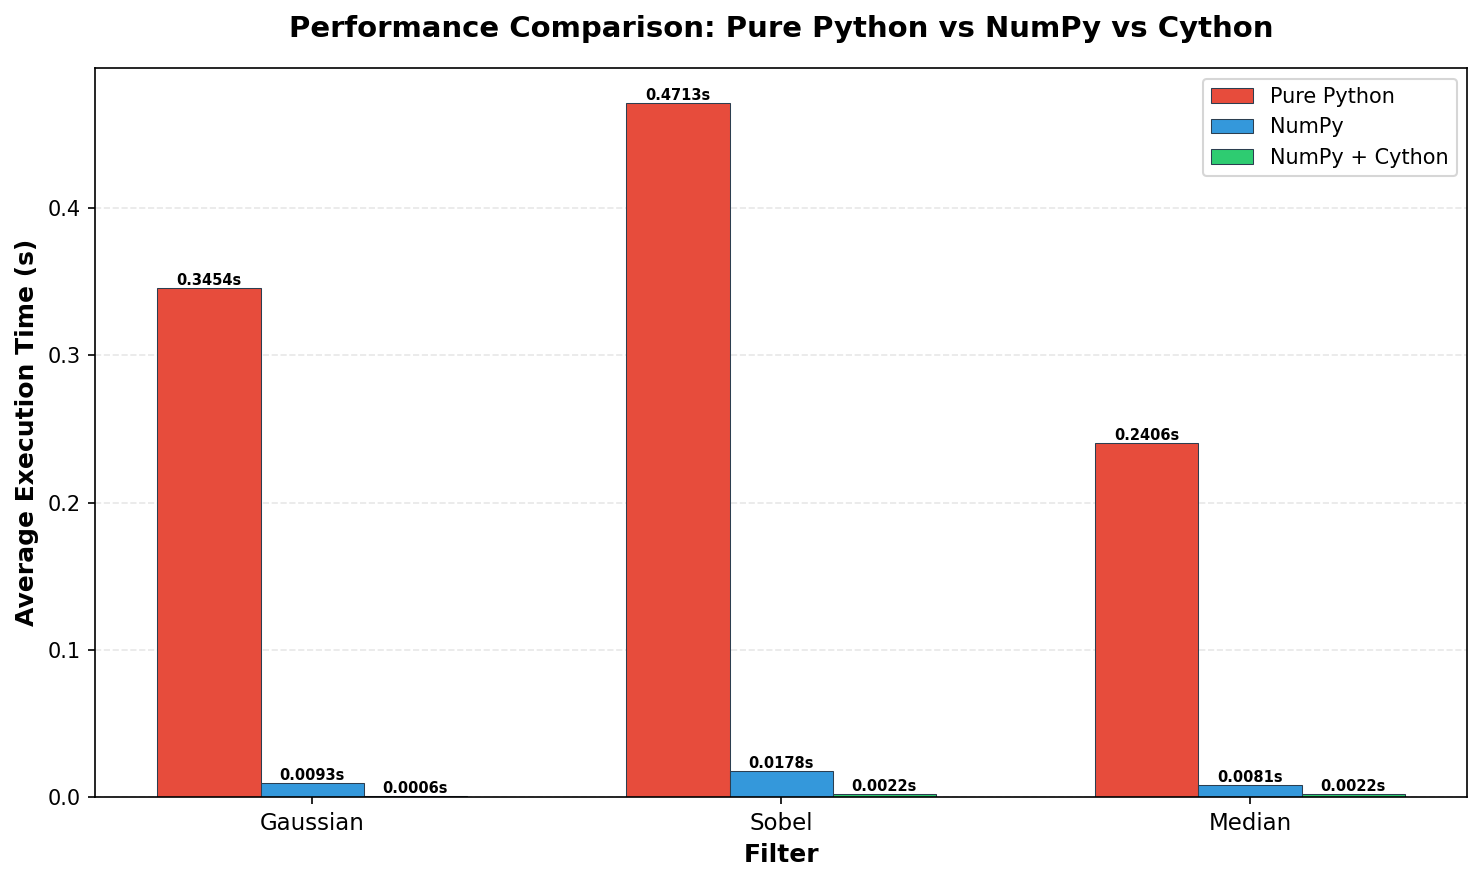
\includegraphics[width=0.85\textwidth]{images/performance_chart.png}
    \caption{Bar chart comparing average execution times across all filter--approach combinations.}
    \label{fig:performance}
\end{figure}

\subsection{Key Observations}

\begin{enumerate}
    \item \textbf{Pure Python is orders of magnitude slower.} The four nested loops for convolution result in heavy Python interpreter overhead per pixel.
    \item \textbf{NumPy achieves 26--37$\times$ speedup} by replacing pixel-level loops with vectorized C operations. The median filter benefits from \texttt{np.median} operating on stacked arrays.
    \item \textbf{Cython delivers 108--612$\times$ speedup} by compiling to C, eliminating Python object overhead, and performing direct memory access through typed buffers. The Gaussian filter sees the largest benefit because its computation is arithmetic-intensive with uniform memory access patterns.
    \item \textbf{Sobel is the most computationally expensive} in Pure Python because it requires two convolutions (X and Y kernels) plus a square root per pixel.
\end{enumerate}

% ══════════════════════════════════════════════════════════════════════
\section{Visual Results}
% ══════════════════════════════════════════════════════════════════════

The following figures show the original image alongside the result of each filter applied using all three approaches. Visually, the filter outputs are identical across approaches---only execution time differs.

\subsection{Gaussian Filter}

\begin{figure}[H]
    \centering
    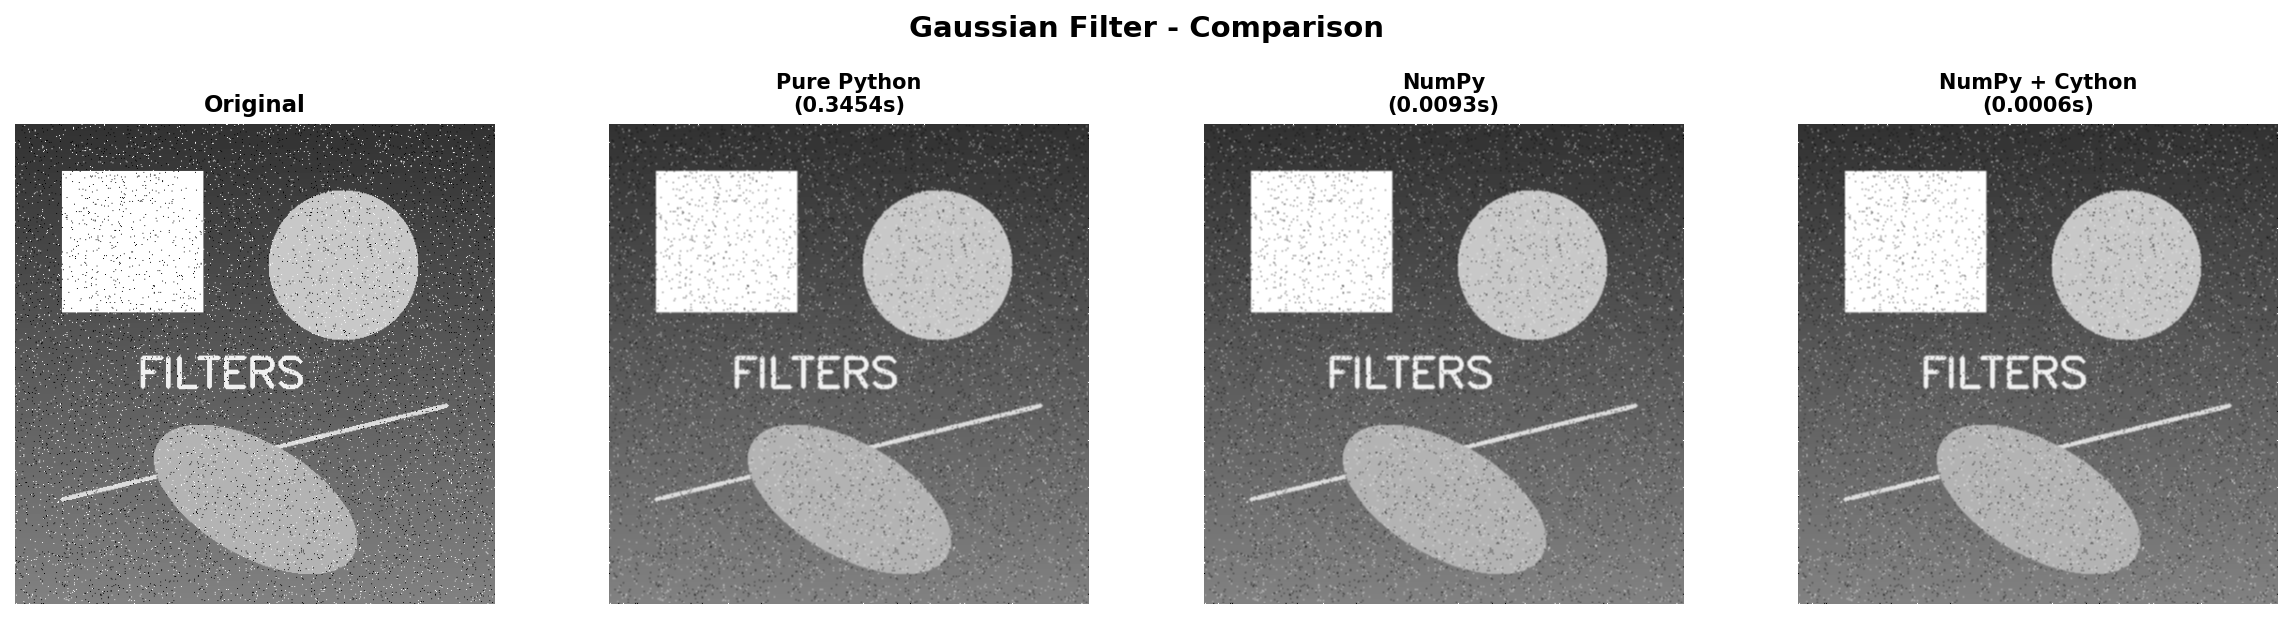
\includegraphics[width=\textwidth]{images/gaussian_comparison.png}
    \caption{Gaussian filter results: Original (left) vs. Pure Python, NumPy, and Cython outputs.}
    \label{fig:gaussian}
\end{figure}

The Gaussian filter produces a smooth, blurred version of the original image. The salt-and-pepper noise present in the original is visibly reduced, and edges become softer.

\subsection{Sobel Filter}

\begin{figure}[H]
    \centering
    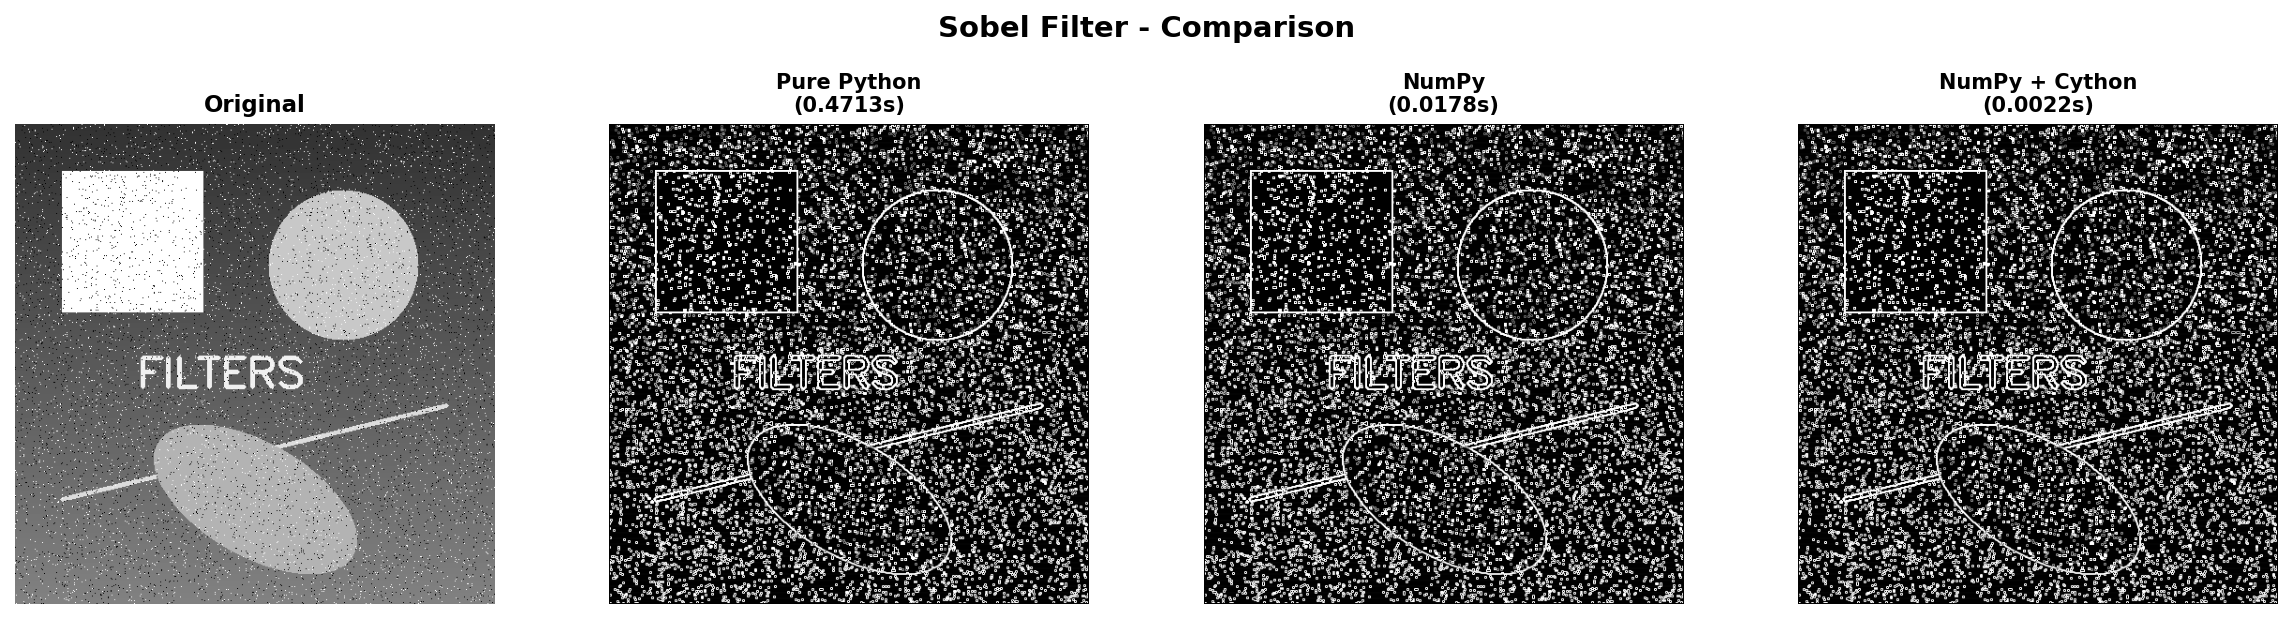
\includegraphics[width=\textwidth]{images/sobel_comparison.png}
    \caption{Sobel filter results: Original (left) vs. Pure Python, NumPy, and Cython outputs.}
    \label{fig:sobel}
\end{figure}

The Sobel filter clearly highlights the edges of all geometric shapes in the test image. The text ``FILTERS'', rectangle, circle, ellipse, and diagonal line are all distinctly outlined against the dark background.

\subsection{Median Filter}

\begin{figure}[H]
    \centering
    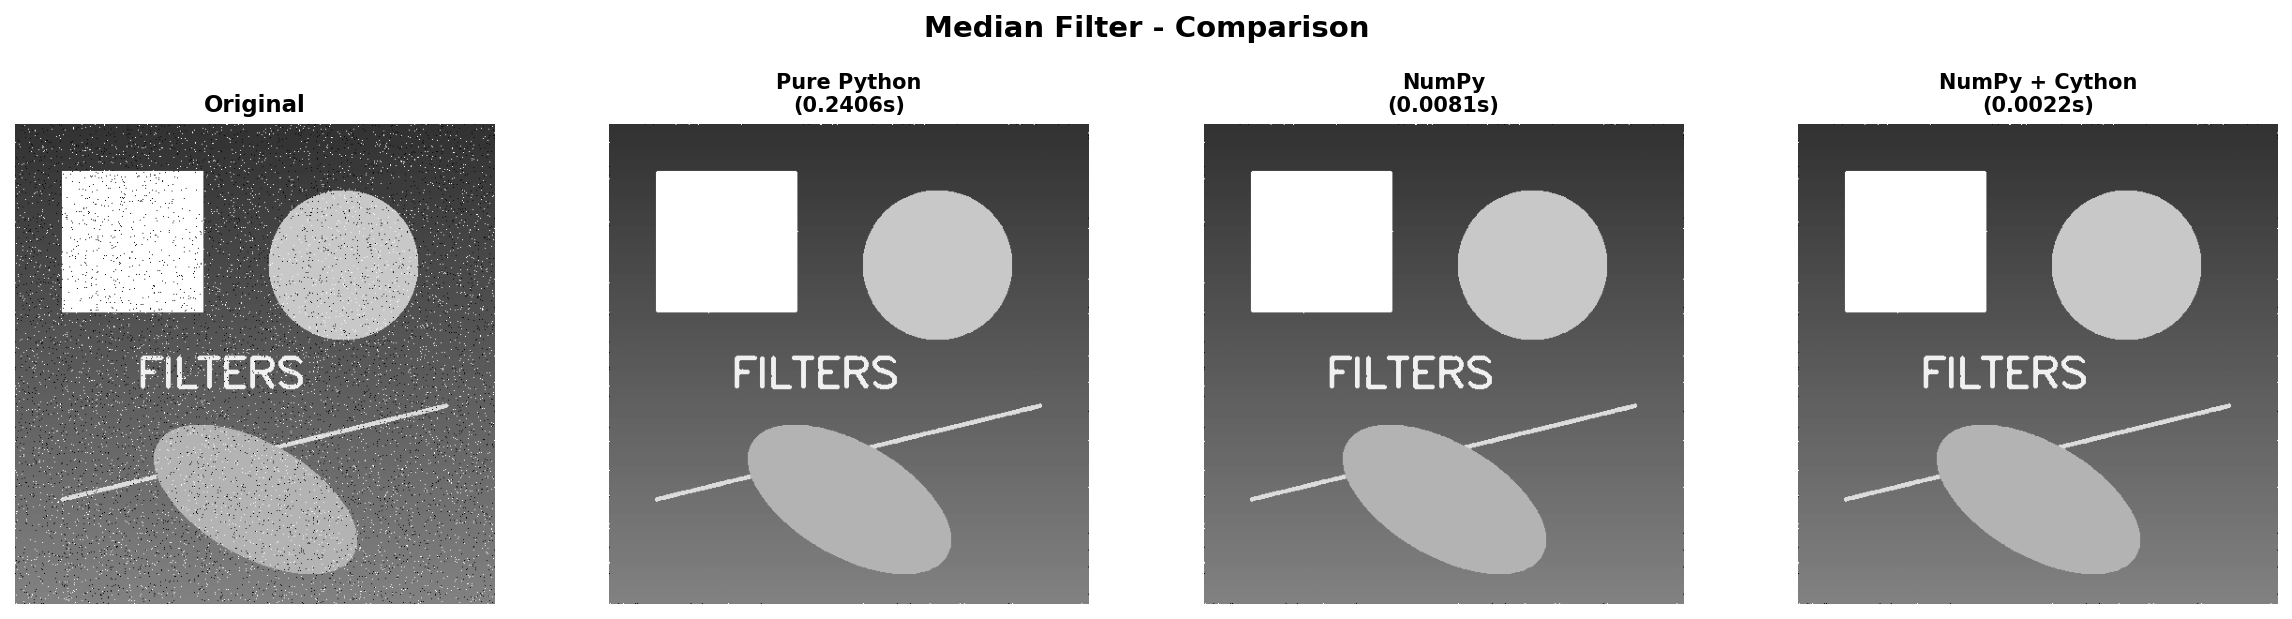
\includegraphics[width=\textwidth]{images/median_comparison.png}
    \caption{Median filter results: Original (left) vs. Pure Python, NumPy, and Cython outputs.}
    \label{fig:median}
\end{figure}

The median filter effectively removes the salt-and-pepper noise while preserving the sharp edges of the shapes. Unlike the Gaussian filter, edges remain crisp---this is the key advantage of median filtering for impulse noise.

% ══════════════════════════════════════════════════════════════════════
\section{Discussion and Conclusions}
% ══════════════════════════════════════════════════════════════════════

\subsection{Trade-offs}

\begin{table}[H]
\centering
\renewcommand{\arraystretch}{1.3}
\begin{tabular}{@{} l c c c @{}}
\toprule
\textbf{Approach} & \textbf{Speed} & \textbf{Ease of Impl.} & \textbf{Setup Complexity} \\
\midrule
Pure Python     & Slowest   & Easiest  & None \\
NumPy           & Fast      & Easy     & \texttt{pip install numpy} \\
NumPy + Cython  & Fastest   & Moderate & C compiler required \\
\bottomrule
\end{tabular}
\caption{Trade-off summary between approaches.}
\end{table}

\subsection{Insights}

\begin{itemize}
    \item \textbf{Pure Python} is adequate for prototyping and small images but becomes impractical for real-time or large-scale image processing. Its primary value is educational: the explicit loops make the algorithm transparent.

    \item \textbf{NumPy} strikes the best balance between performance and developer productivity. With a single \texttt{pip install}, it achieves 26--37$\times$ speedup with minimal code complexity. For most practical applications, NumPy is the recommended choice.

    \item \textbf{Cython} is justified when extreme performance is critical, such as processing video streams or very high-resolution images. The 100--600$\times$ speedup comes at the cost of needing a C compiler and writing slightly more verbose code with type annotations.

    \item The \textbf{diminishing returns} from NumPy to Cython depend on the filter type. Arithmetic-heavy operations (like Gaussian convolution) benefit the most from Cython's compiled arithmetic. The median filter, which relies on sorting, shows a smaller (but still substantial) improvement because the bottleneck shifts from Python overhead to algorithmic complexity.
\end{itemize}

\subsection{Conclusion}

This project demonstrates that computational optimization can dramatically accelerate image processing operations. By transitioning from Pure Python to NumPy and then to Cython, we achieved speedups of up to $612\times$ while maintaining identical output quality. The choice of approach should be guided by the application's performance requirements and development constraints.

\end{document}
